\underline{Muster 1: identische Startsequenz}
\newline
Dieser Ausrutscher passiert, wenn eine Sequenz sehr 
viel vertrauter ist als die andere Sequenz, sie aber 
die gleiche Startsequenz haben und man so oft in die 
falsche Sequenz 'überläuft'.

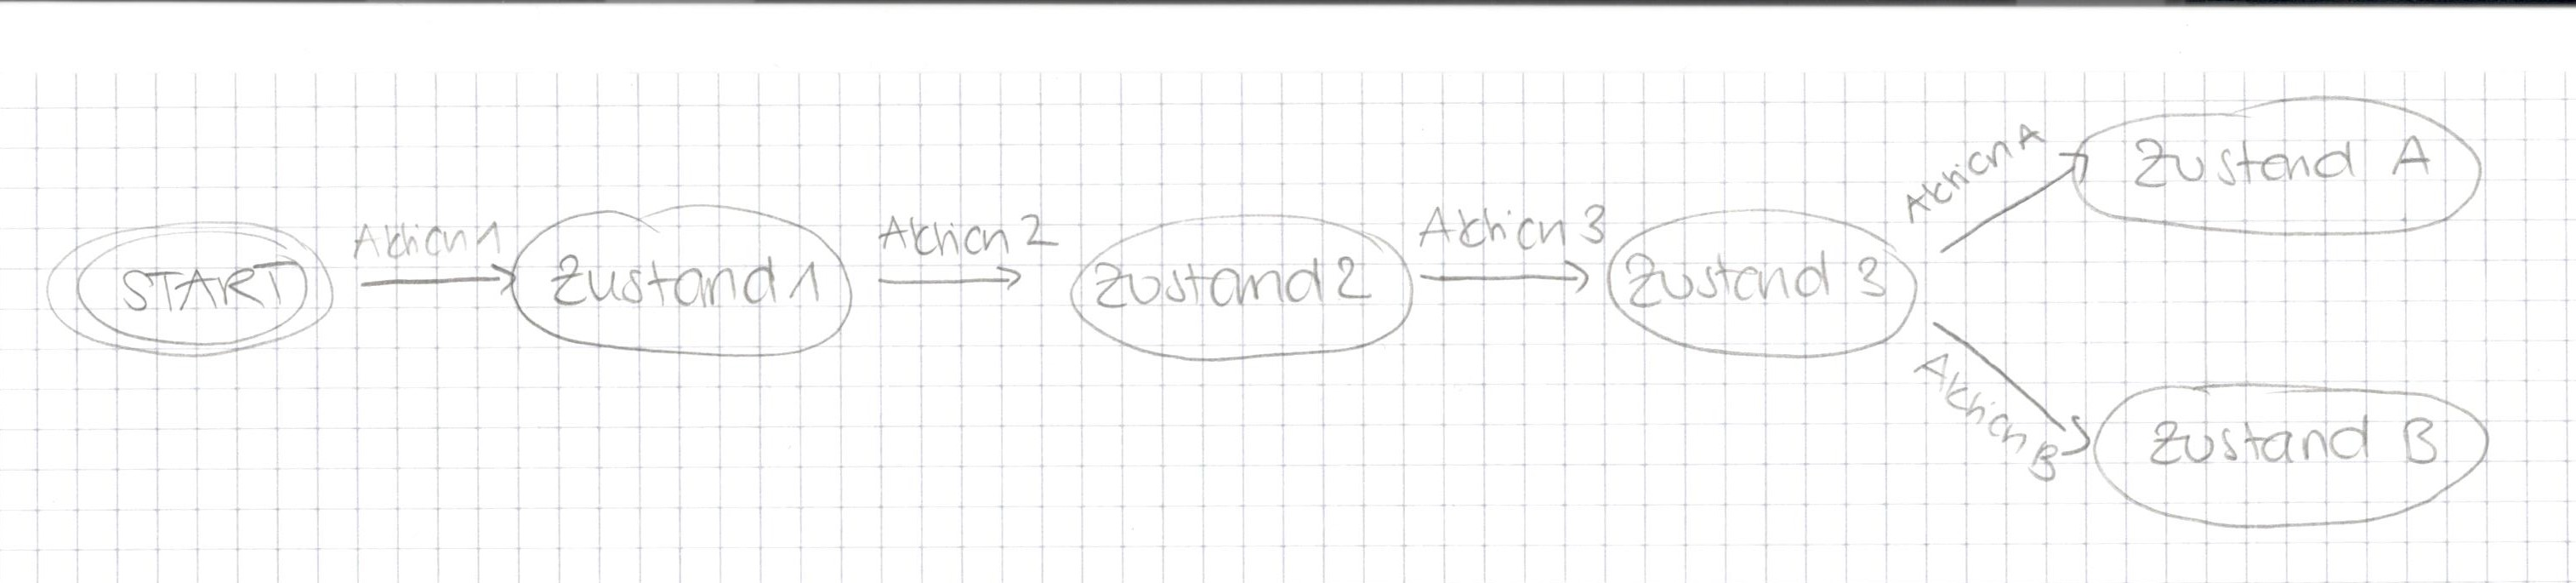
\includegraphics[scale=.5]{images/Muster1.jpeg}

\underline{Muster 2: Closure}
\newline
Das Gefühl von Closure kommt bei diesem Ausrutscher zu 
früh und führt somit zum Abbrechen der Sequenz obwohl 
sie noch nicht zu Ende ist. (Wie am Beispiel der älteren 
Geldautomaten)

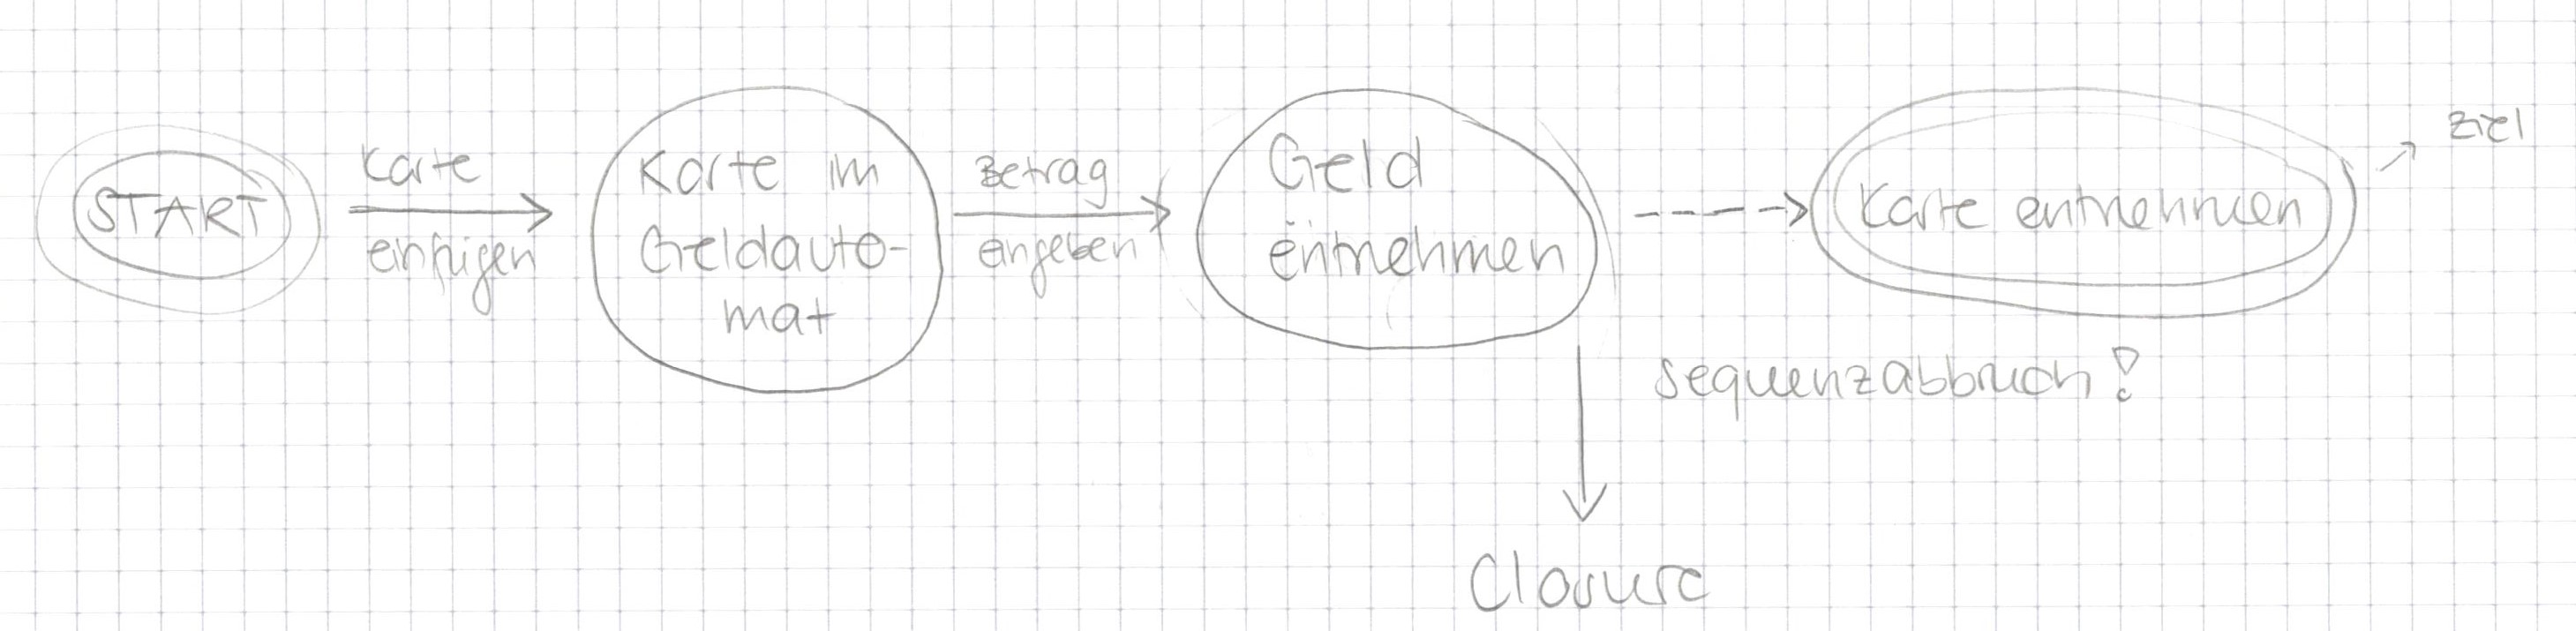
\includegraphics[scale=.5]{images/Muster2.jpeg}

\underline{Muster 3: Das Kurzzeitgedächtnis ist überladen}
\newline
Bei diesem Ausrutscher werden gewisse Handlungsstufen 
oder sogar das Ziel vergessen, weil man es nicht schafft, 
sich alle zu merken, da es zu viele Schritte hat bis man am 
Ziel angelangt.

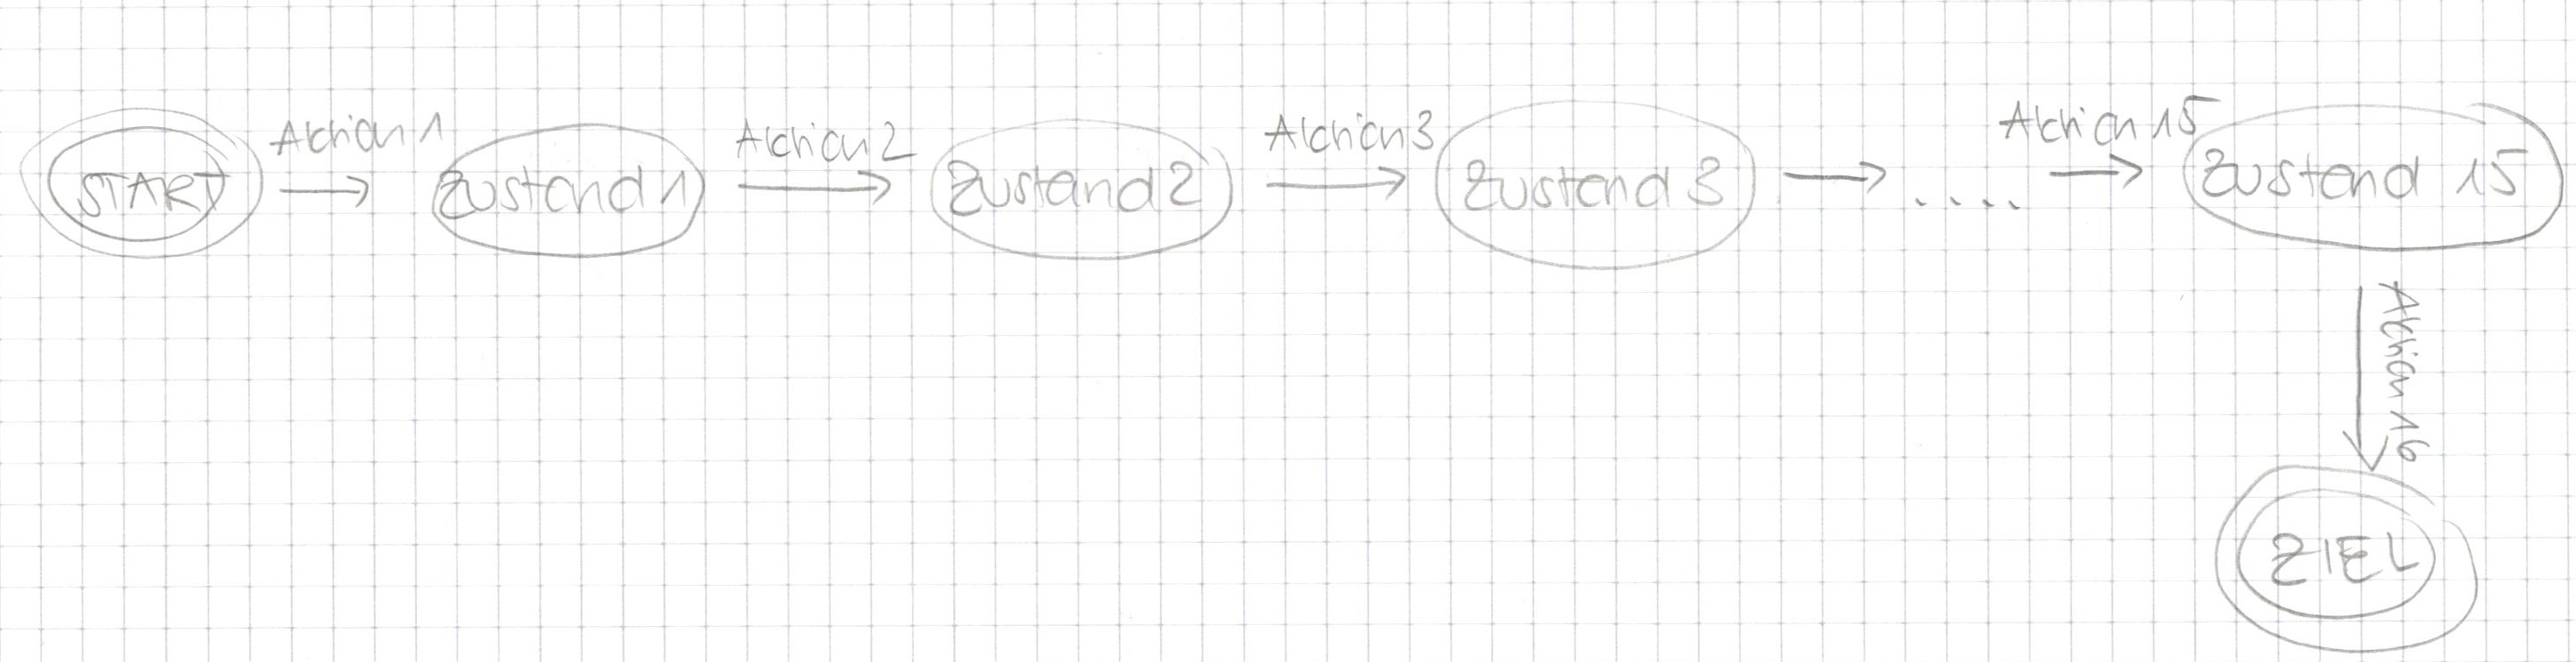
\includegraphics[scale=.5]{images/Muster3.jpeg}
